\section{Points of presence (POPs)}

A point of presence (PoP) is an artificial demarcation point or interface point between communicating entities.
In our case we are refering to optical fibre interconnection points.
From 2010 until now the guifi.net community has raised six points of presence over the Catalan territory.
This POPs are following the network model of freedom and neutrality specified in the XOLN\ref{XOLN} licence.
Thus anyone is able to connect to them but always respecting the same conditions.
From a general perspective guifi.net community is building a set of neutral exchange points, leaving the
infraestructure available to the individuals, associations or either companies.

Figure \ref{fig:fibre_map} shows the fibre network map of guifi.net (not all of them).

\begin{figure}[htbp]
  \centering
  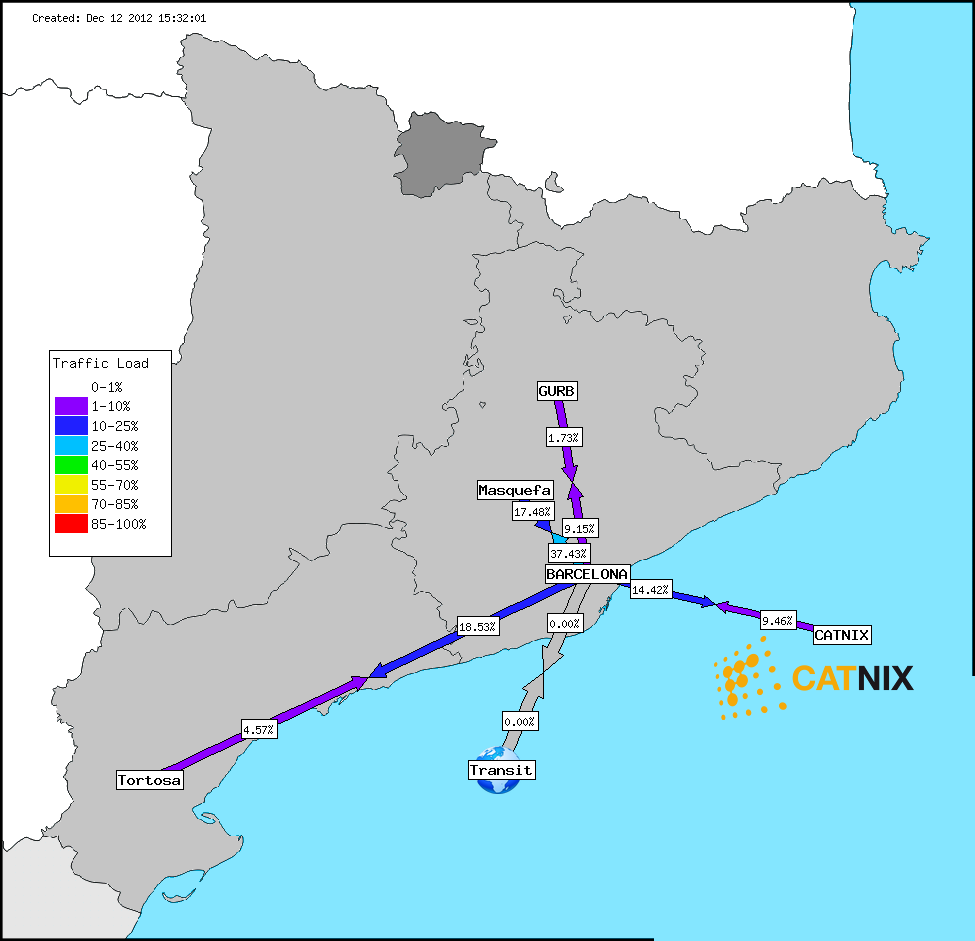
\includegraphics[scale=.35]{sect3/figures/pops_network_map.eps} %% use convert command to convert formats "convert pops_network_map.png pops_network_map.eps" e.g. 
  \caption{Guifi.net fibre network map}
  \label{fig:fibre_map}
\end{figure}



\subsection{Pilot's deployments}

\subsubsection{Gurb}

\subsubsection{Vic}


\subsection{Other deployments}


